\chapter{Конструкторский раздел}

В данном разделе сформулированы требования и ограничения к разрабатываемому методу. Разработан метод повышения разрешения изображения по нескольким кадрам. Описаны основные этапы разработки в виде детализированной диаграммы IDEF0 и схем алгоритмов, а также изложены особенности предлагаемого метода. Спроектировано программное обеспечение для реализации разрабатываемого метода.

\section{Требования и ограничения к разрабатываемому методу}

К методу повышения разрешения изображения по нескольким кадрам предъявляются следующие требования:

\begin{enumerate}
    \item Метод должен базироваться на использовании сверточных нейронных сетей с необходимыми модификациями.
    \item Метод должен подавлять шум, присутствующий в отдельных кадрах, не теряя при этом полезные детали.
    \item Метод должен сохранять и улучшать мелкие детали (не только увеличивать размер изображения).
    \item Метод должен быть применим для работы с различными типами объектов и сцен, а также различными освещением.
\end{enumerate}

Также представлен ряд ограничений для разрабатываемого метода:

\begin{enumerate}
    \item Качество восстановления может быть неудовлетворительным, если входные изображения подвержены критичному искажению или некачественно зарегистрированы фотосистемой.
    \item Качество восстановления может быть неудовлетворительным, если входные изображения с высоким уровнем шума и/или имеют высокочастотные детали (выбросы интенсивности).
\end{enumerate}

\section{Требования к разрабатываемому программному обеспечению}

К разрабатываемому программному обеспечению предъявляются следующие требования:

\begin{enumerate}
    \item Возможность загрузки изображений в формате PNG, JPG или BMP.
    \item Возможность обработки как RGB~--~изображений, так и изображений в тонах серого.
    \item Возможность просмотра результата повышения разрешения изображения.
    \item Возможность просмотра информации по процессу обучения модели.
    \item Возможность просмотра значения выбранных метрик качества для конкретного случая работы алгоритма.
    \item Возможность сохранения результата в отдельный файл в формате PNG, JPG или BMP.
    \item Если время выполнения программы может превышать комфортное время реакции системы для человека, необходимо обеспечить вывод предупреждающего сообщения. 
    \item Разрабатываемое ПО должно корректно реагировать на любые действия пользователя.
\end{enumerate}

\clearpage

\section{Основные этапы разрабатываемого метода}

\subsection{IDEF0~--~диаграмма уровня А0}

На рисунке \ref{idef0-a0} представлена IDEF0~--~диаграмма уровня А0 для метода повышения разрешения изображения по нескольким кадрам.

\begin{figure}[H]
    \centering
    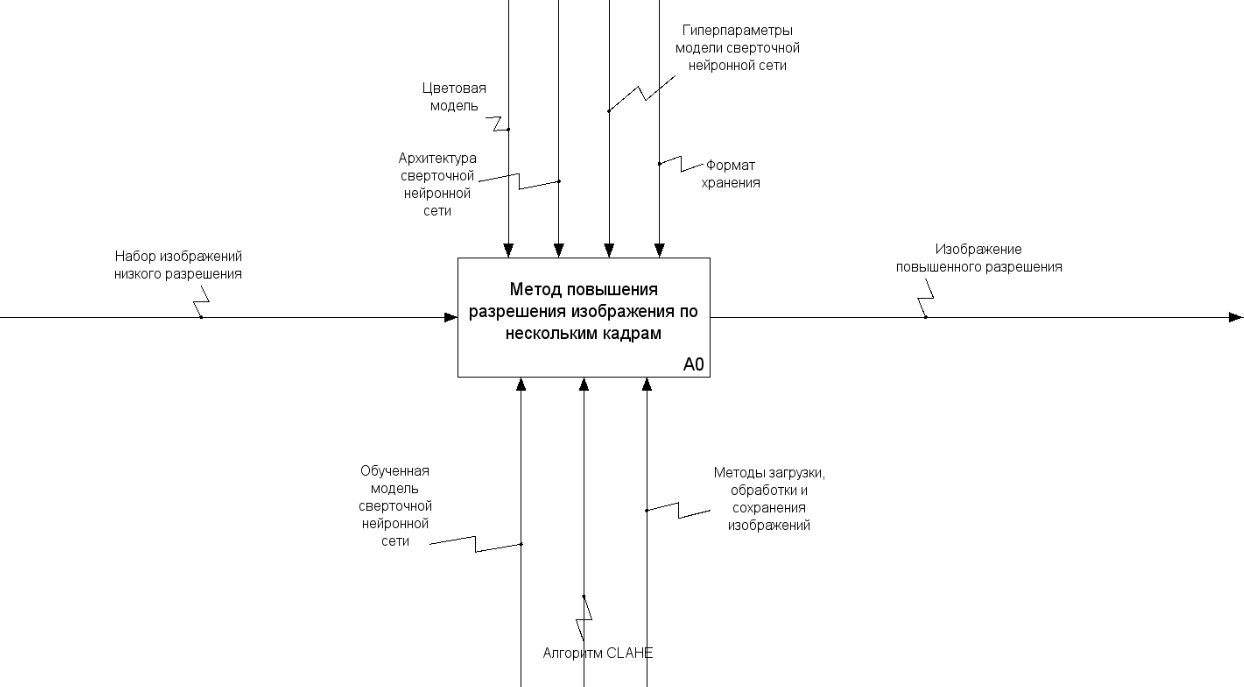
\includegraphics[scale=0.45]{assets/idef0-a0.png}
    \caption{IDEF0~--~диаграмма уровня А0}
    \label{idef0-a0}
\end{figure}

На рисунке \ref{idef0-a1} представлена детализированная IDEF0~--~диаграмма для метода повышения разрешения изображения по нескольким кадрам.

\begin{figure}[H]
    \centering
    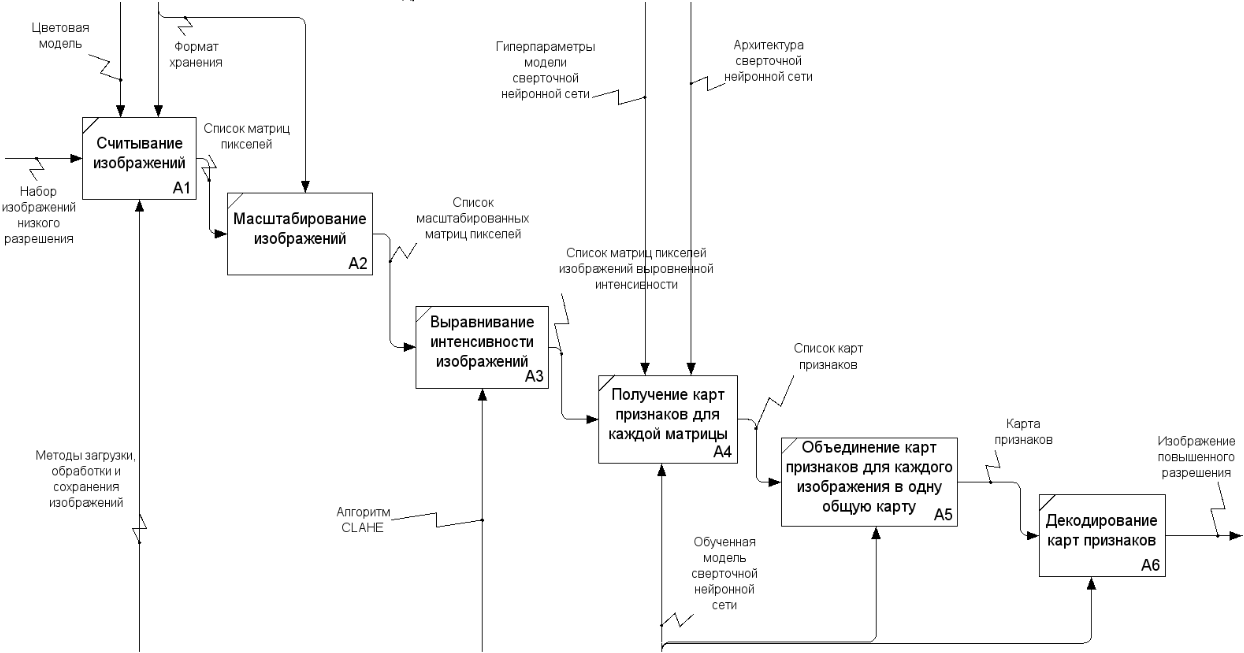
\includegraphics[scale=0.5]{assets/idef0-a1.png}
    \caption{IDEF0~--~диаграмма уровня А1}
    \label{idef0-a1}
\end{figure}

Особенностью рассматриваемой архитектуры нейронной сети является обработка нескольких входных изображений (в отличии от одного для классической архитектуры), в связи с чем обработка входного набора изображений также требует дополнительных действий (приведение к одному размеру, выравнивание интенсивности кадров низкого разрешения, конкатенация карт признаков нескольких кадров).

\subsection{Алгоритм обработки входных изображений}

На рисунке \ref{data-proc} представлен алгоритм обработки входных изображений (кадров низкого разрешения).

\begin{figure}[H]
    \centering
    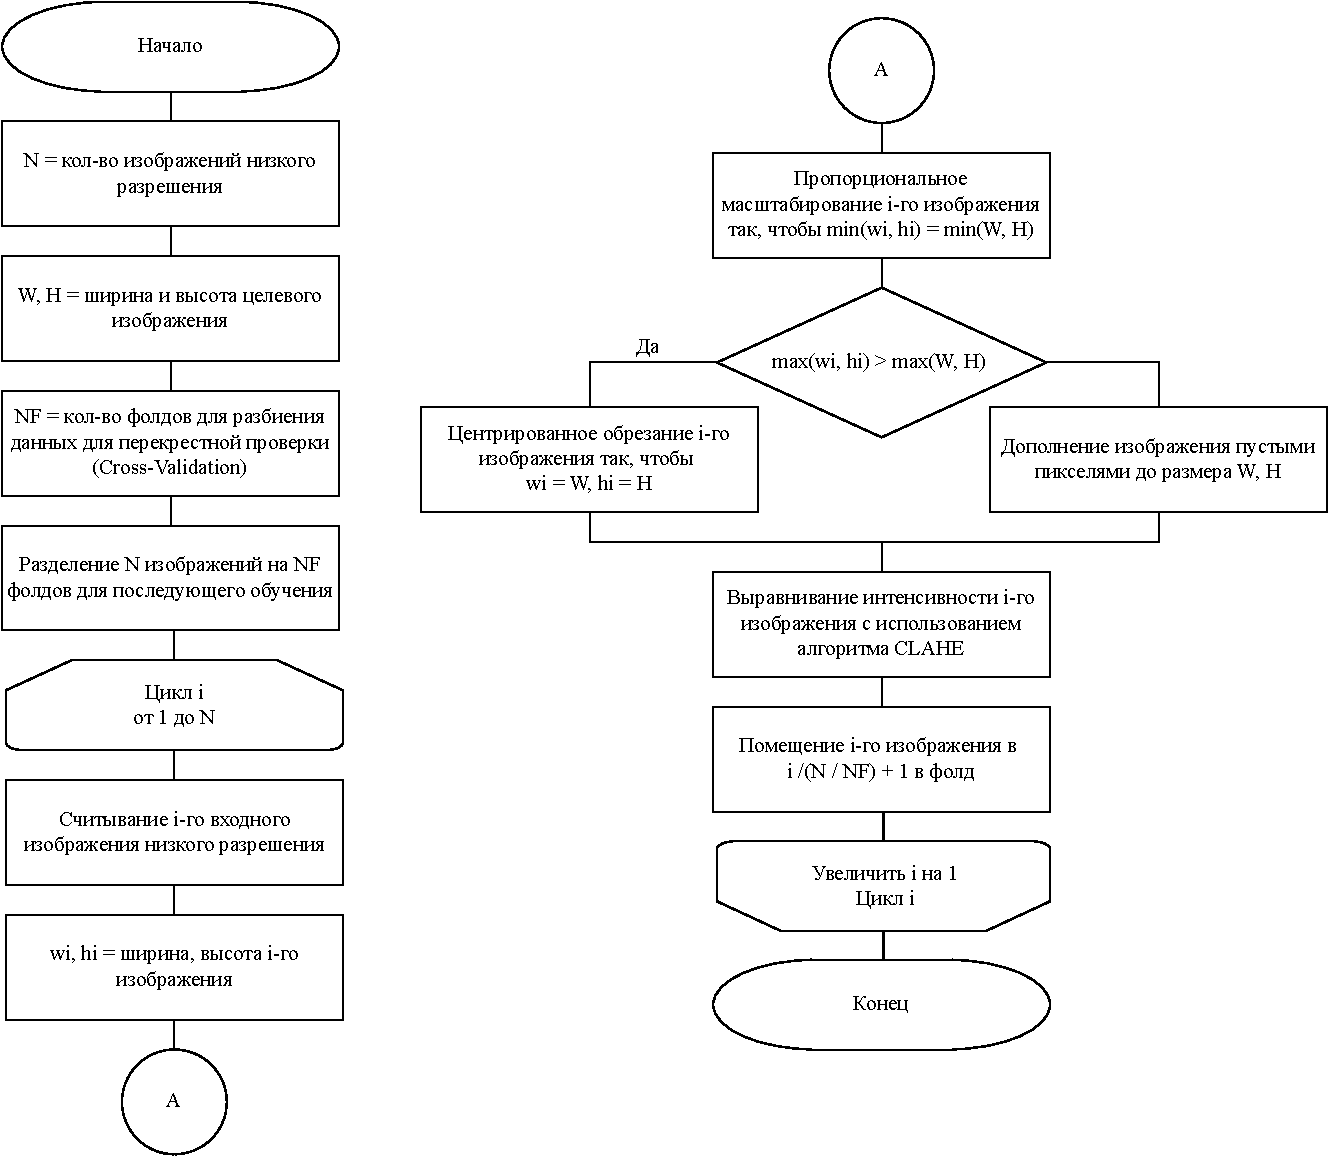
\includegraphics[scale=0.75]{assets/data_processing.pdf}
    \caption{Алгоритм обработки входных изображений}
    \label{data-proc}
\end{figure}

\subsection{Алгоритм констрастно~--~ограниченной эквализации гистограммы}

На рисунке \ref{clahe} представлен алгоритм констрастно~--~ограниченной эквализации гистограммы (CLAHE --- англ. Contrast Limited Adaptive histogram equalization), применяемый к каждому входному изображению с целью улучшения видимости деталей в затемненных или засвеченных областях изображения, предотвращая при этом чрезмерное усиление шума.

\begin{figure}[H]
    \centering
    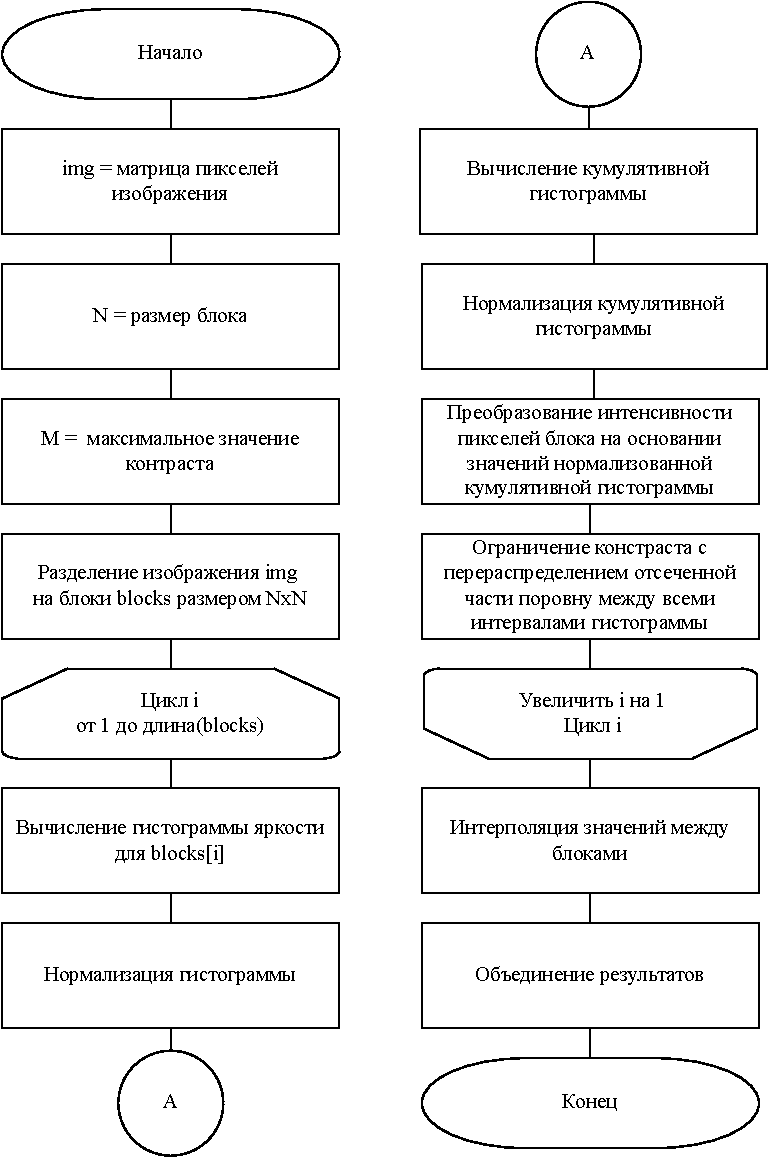
\includegraphics[scale=0.9]{assets/clahe}
    \caption{Алгоритм констрастно~--~ограниченной эквализации гистограммы}
    \label{clahe}
\end{figure}

В обычной адаптивной гистограммной эквализации (AHE) контраст может быть увеличен до такой степени, что небольшие вариации интенсивности, включая шум, становятся сильно заметными, ухудшая качество изображения. CLAHE решает эту проблему, ограничивая усиление контраста в каждой локальной области, что позволяет улучшить видимость деталей без значительного увеличения шума и артефактов.

На рисунке \ref{clahe-example} представлен пример применения алгоритма CLAHE.

\begin{figure}[H]
    \centering
    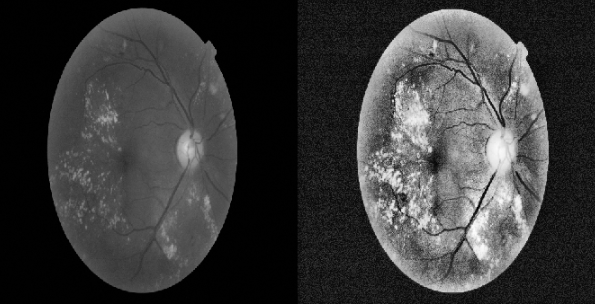
\includegraphics[scale=0.95]{assets/clahe-example}
    \caption{Пример применения алгоритма CLAHE}
    \label{clahe-example}
\end{figure}

\subsection{Свертка (конволюция)}

Применительно к обработке цифровых изображений операция свертки может быть интерпретирована следующим образом: на основе некоторого множества пикселей исходного изображения вычисляется новый пиксель результирующего (искаженного ядром свертки) изображения.

В зависимости от выбранного ядра свертки, применяемого к изображению, можно получить тот или иной эффект: размытость, повышение резкости, обнаружение контуров, граничное обнаружение и т.~д.

Математически операцию двумерной свертки цифрового изображения размером $M \times N$ в пространственной области можно описать в виде выражения~(\ref{svertka})~\cite{svertka}: 
\begin{equation}\label{svertka}
	f(x,\;y) \oplus h(x,\;y) = \frac{1}{MN}\sum_{m=0}^{M-1}\sum_{n=0}^{N-1} f(m,\;n) \cdot h(x - m,\;y - n).
\end{equation}

На рисунке \ref{conv}~\cite{conv} представлен пример выполнения операции свертки. Для вычисления новых значений используется т.н. ядро свертки. На представленном примере ядром является матрица серого цвета размером $3\times3$ ячейки.

\begin{figure}[H]
    \centering
    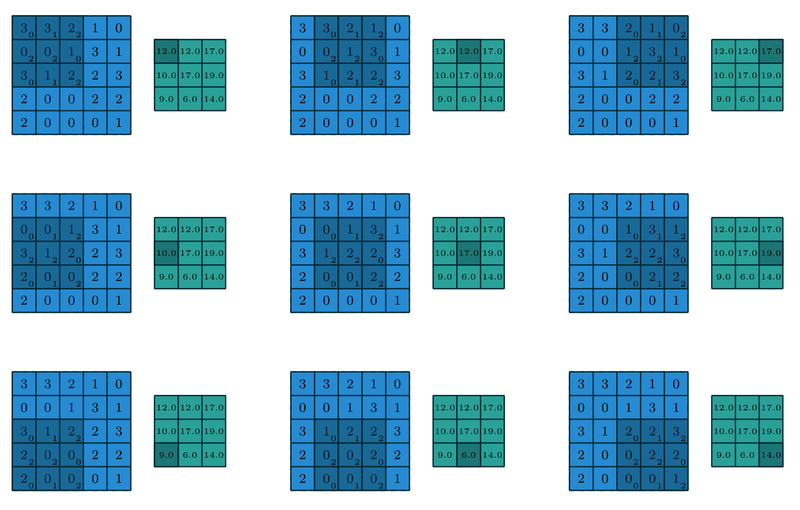
\includegraphics[scale=1.4]{assets/convolution_example}
    \caption{Пример конволюции цифрового изображения}
    \label{conv}
\end{figure}

Использование свертки в рамках рассматриваемой задачи предоставляет инструмент для извлечения высокоуровневых характеристик изображения, которые затем используются для повышения разрешения целевого изображения посредством составления различных карт характеристик, т.е. применения сверток с различными ядрами, описывающими то или иное свойство. Начальные значения весов нейронов в сети задаются случайным образом. Начальные значения весов нейронов в сети задаются случайным образом. Обычно сверточный слой по умолчанию объединяется с нелинейной функцией активации~\cite{layers}.

После применения сверточного слоя также часто применяются подвыборочные слои с целью уплотнения карты признаков: считается, что обнаружение признака важнее нахождения его координат. Таким образом, карты признаков после прохождения нескольких слоев сети могут преобразоваться в вектор или скаляр.

\subsection{Алгоритм конкатенации карт признаков}

На рисунке \ref{data-proc} представлен алгоритм конкатенации карт признаков.

\begin{figure}[H]
    \centering
    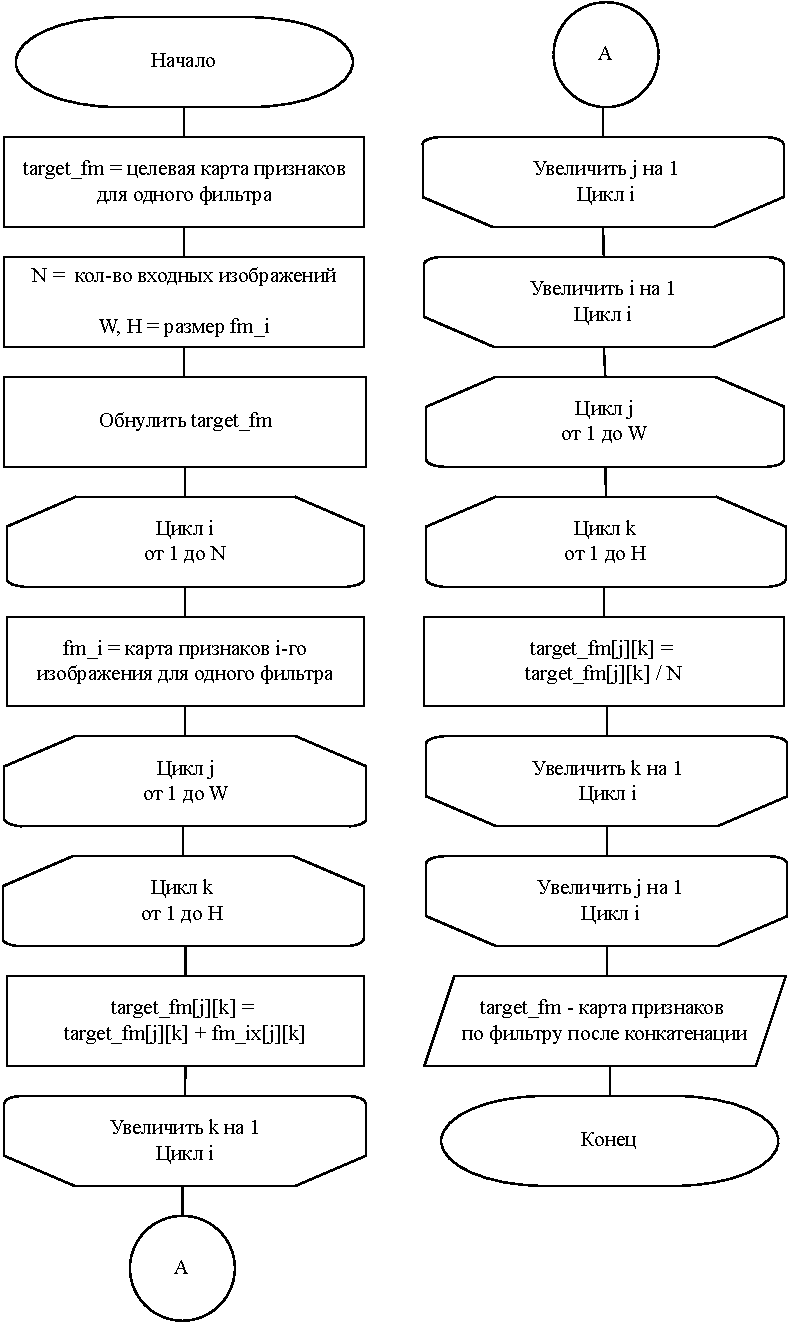
\includegraphics[scale=1]{assets/concat.pdf}
    \caption{Алгоритм конкатенации карт признаков}
    \label{data-proc}
\end{figure}

\clearpage

\subsection{Архитектура разрабатываемой нейронной сети}

На рисунке \ref{model} представлена базовая архитектура \cite{train3, train4} разрабатываемой нейронной сети на данный момент.

\begin{figure}[H]
    \centering
    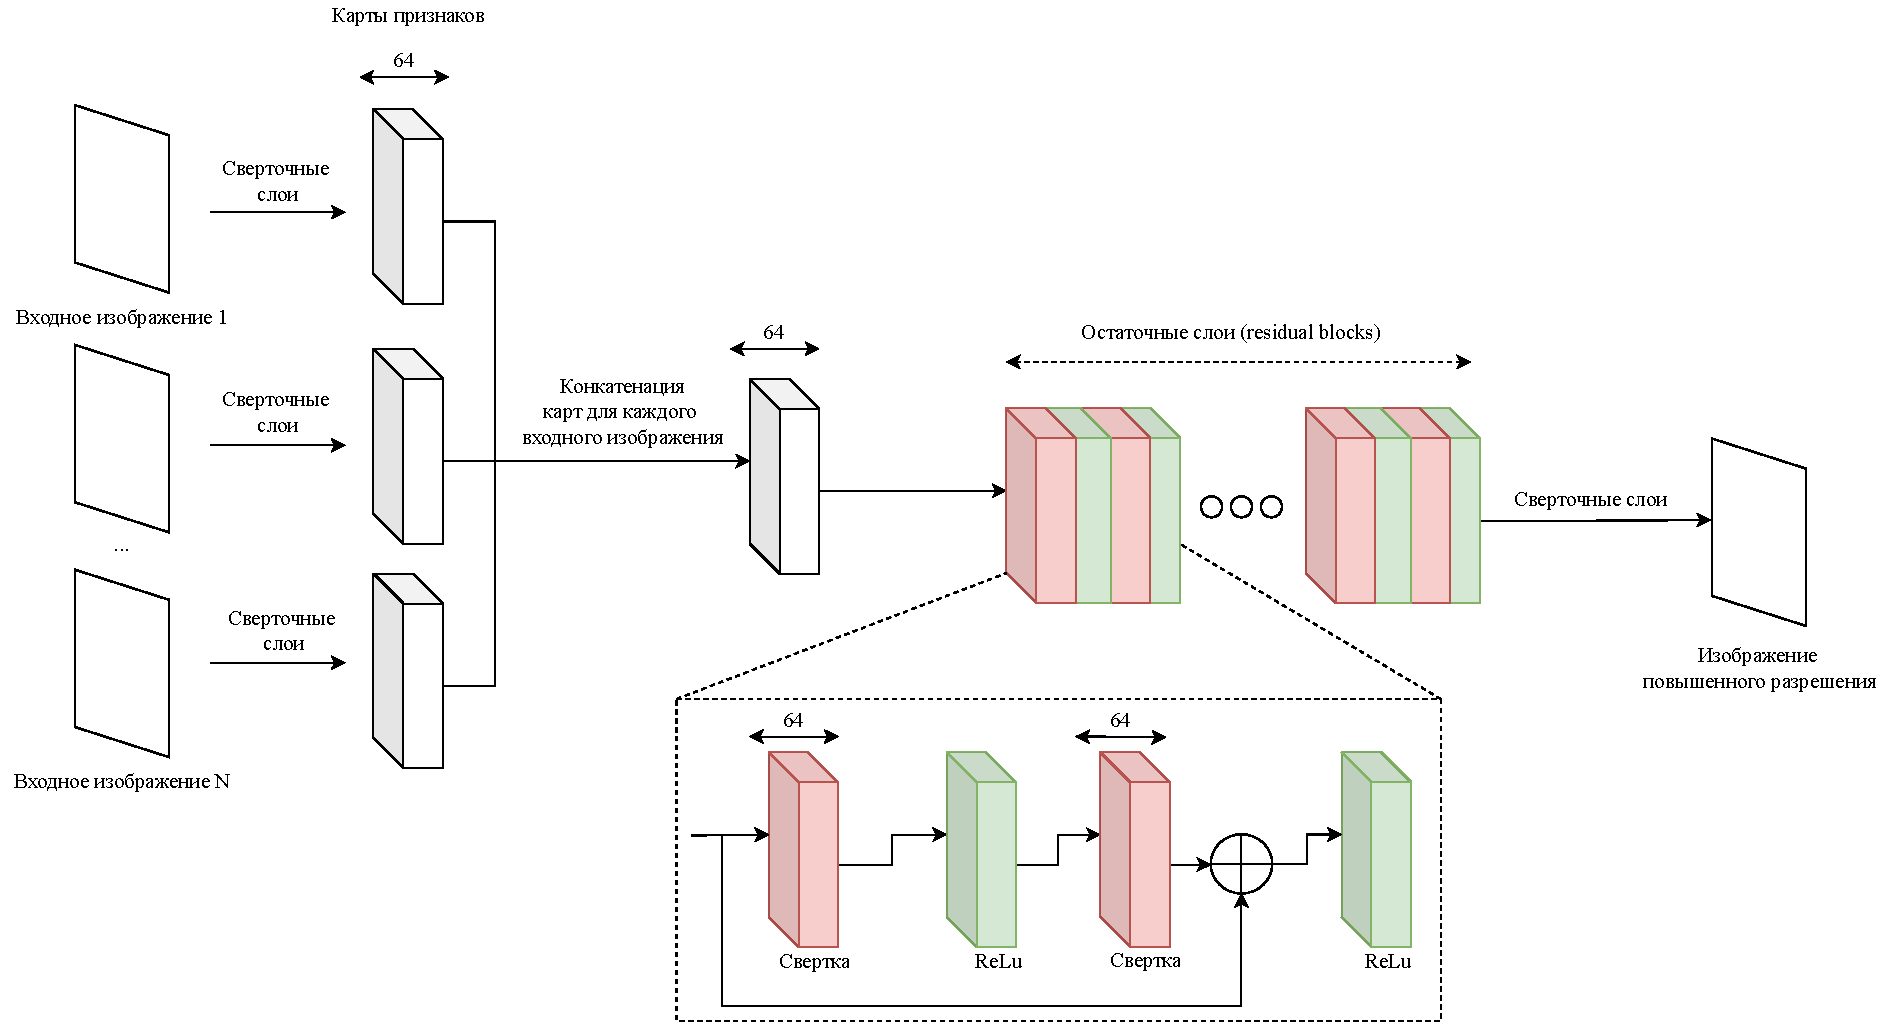
\includegraphics[scale=0.5]{assets/model.pdf}
    \caption{Базовая архитектура разрабатываемой нейронной сети для задачи суперразрешения}
    \label{model}
\end{figure}

В настоящее время для обучения нейронных сетей, в том числе глубоких, используется алгоритм обратного распространения ошибки (англ. error backpropagation algorithm), основанный на методе градиентного спуска. 

Сверточная нейронная сеть не имеет обратных связей и является многослойной~\cite{layers2}.

В глубокой нейронной сети с несколькими скрытыми слоями производится расчет ошибки, которая передается от одного слоя к другому. На первом этапе рассчитывается значение ошибки на выходе нейронной сети, для которого известны правильные ответы. Затем рассчитывается ошибка на входе в выходной слой сети, которая будет использоваться как ошибка на выходе скрытого слоя~\cite{train2, train}.

Для решения проблемы затухающего градиента во время обучения используется подход использования остаточных блоков (англ. residual blocks~\cite{residual}): входной сигнал пропускается не только через обычные слои, но и напрямую добавляется к выходу этих слоёв, обходя один или несколько слоёв, т.о. создавая короткий путь для градиентов во время обратного распространения.

\subsection{Структура разрабатываемого программного обеспечения}

На рисунке \ref{struct-po} представлена диаграмма компонентов \cite{uml} разрабатываемого программного обеспечения.

\begin{figure}[H]
    \centering
    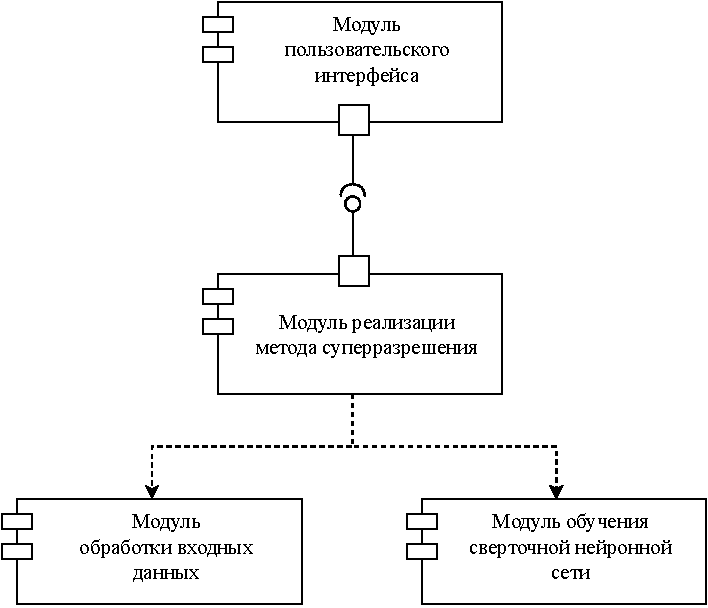
\includegraphics[scale=1]{assets/struct_po.pdf}
    \caption{Диаграмма компонентов разрабатываемого программного обеспечения}
    \label{struct-po}
\end{figure}

\section{Методы оценки качества восстановления цифрового изображения}

Существует несколько методов оценки качества восстановленного изображения \cite{metrics, metrics2}:

\begin{itemize}
    \item \textit{Среднеквадратичная ошибка} (англ. MSE --- Mean Square Error) --- наиболее широко используемый, а также самый простой полный эталонный показатель, который рассчитывается как квадрат разности интенсивностей пикселей искаженного и эталонного изображения:

    $\textbf{MSE}(f, g) = \displaystyle\cfrac{1}{MN}\sum_{i=1}^{M}\sum_{j=1}^{N} (f_{ij} - g_{ij}) ^ 2,$ где $f$ и $g$ --- целевое и восстановленное изображения, $M, N$ - размер изображения.
    
    Встречается также вариация метрики --- корень из MSE (англ. RMSE Root Mean Square Error). 
    
    \item \textit{Пиковое отношение сигнал~--~шум} (англ. PSNR --- Peak Signal--to--Noise Ratio) --- скалярная метрика, обозначающая соотношение между максимальной мощностью сигнала и шума. Для вычисления PSNR чаще всего используется среднеквадратичная ошибка (англ. Mean Square Error). Метрика выражается в логарифмической шкале и измеряется в децибелах: $\textbf{PSNR}(f, g) = \displaystyle 10\cdot \log_{10} \cfrac{255^2}{MSE(f, g)}$.
    
    Является основным количественным критерием для оценки эффективности восстановления сигналов в виду, однако имеет ряд ограничений, основным из которых является тот факт, что PSNR (и MSE в частности) слабо коррелируют с физиологией человеческого восприятия.
    
    \item \textit{Индекс SSIM }(англ. Structure Similarity Index) характеризует структурное сходство между оригинальным и восстановленным сигналами, принимает значение в диапазоне от -1 до 1, где 1 соответствует совпадению оригинального сигнала с восстановленным, а -1 --- полному различию сигналов. Метрика учитывает яркость, контрастность и структуру изображения. 
    
    Метрика может быть вычислена согласно следующей формуле: $\textbf{SSIM}(f, g) = [l(f, g)]^\alpha\cdot[c(f, g)]^\beta\cdot[s(f, g)]^\gamma$, где $l$ --- яркость (используется для сравнения яркости между двумя изображениями), $c$ --- контраст (используется для различия диапазонов между самой яркой и самой темной областью двух изображений), $s$ --- функция сравнения структур, которая измеряет коэффициент корреляции между двумя изображения, а $\alpha, \beta, \gamma$ --- положительные константы.

    \item\textit{ Метрика оценки восприятия человека} (англ. HPM --- Human Perception Metric) характеризует качество восстановленного сигнала на основе психофизиологических особенностей восприятия сигналов человеком. Является наиболее трудозатратной, т.к. требует участие людей в проведении эксперимента и анализе данных, однако является наиболее достоверной.
\end{itemize}